% Engineering style guide LaTeX template
% Created by Josh Jeppson
% You are free to distribute and use this template as long as I am given credit
% Maybe it will make my job of grading your papers easier

\documentclass[letterpaper]{report}
\usepackage{fancyhdr}
\usepackage{tcolorbox}
\usepackage{layout}
\usepackage[margin=1in]{geometry}
\usepackage{pgf}
\usepackage{pgfpages}
\usepackage{pgfplots}
\usepackage{graphicx}
\usepackage{amsfonts}
\usepackage{amsmath}
\usepackage{amssymb}
\usepackage{tikz,pgfplots}
\usepackage[abspage,user,lastpage]{zref}
\usepackage{lastpage}
\usepackage{marginnote}
\usepackage{eso-pic}
\usepackage{ulem}
\usepackage{tikz}
\usepackage{circuitikz}
\usepackage{wrapfig}
\usepackage[export]{adjustbox}
\usepackage{listings}
\usepackage{xcolor}
\usepackage{soul}
\usepackage{cite}
\usepackage{url}
\usepackage[absolute]{textpos}
\usepackage{amssymb}  % provides Rbb, etc.
\usepackage{latexsym}  % provides \Box
\usepackage{array}
% \usepackage{forest}

\pgfplotsset{compat=1.18}

\usetikzlibrary{plotmarks}
\usetikzlibrary{arrows}
\usetikzlibrary{patterns}
\usetikzlibrary{shapes.geometric}
\usetikzlibrary{shapes.arrows}
\usetikzlibrary{decorations}
\usetikzlibrary{decorations.pathreplacing}
\usetikzlibrary{positioning}

\definecolor{codegreen}{rgb}{0,0.6,0}
\definecolor{codegray}{rgb}{0.5,0.5,0.5}
\definecolor{codepurple}{rgb}{0.58,0,0.82}
\definecolor{backcolour}{rgb}{0.95,0.95,0.92}

\lstdefinestyle{mystyle}{
	backgroundcolor=\color{white},
	commentstyle=\color{green},
	keywordstyle=\color{blue},
	numberstyle=\tiny\color{codegray},
	stringstyle=\color{red},
	basicstyle=\ttfamily\footnotesize,
	breakatwhitespace=false,
	breaklines=true,
	captionpos=b,
	keepspaces=true,
	numbers=left,
	numbersep=5pt,
	showspaces=false,
	showstringspaces=false,
	showtabs=false,
	tabsize=2
}
\lstset{style=mystyle}

\allowdisplaybreaks

\usetikzlibrary{arrows.meta}

% ROBDD Style
% \forestset{
%   BDT/.style={
%     for tree={
%       if n children=0{}{circle},% use a circle unless there are 0 children
%       draw,% draw every node
%       edge={
%         my edge,% use the my edge style for edges (with the arrow)
%       },
%       if n=1{
%         edge+={0 my edge},% if the child is the first one, add the 0 my edge style (dashed)
%       }{},
%       font=\sffamily,% use sans serif for node text
%     }
%   },
% }

\usetikzlibrary{calc, positioning, tikzmark}

\newcommand\BackgroundPic{%
\put(0,0){%
\parbox[b][\paperheight]{\paperwidth}{%
\vfill
\centering
\includegraphics[width=\paperwidth,height=\paperheight,%
keepaspectratio]{background.jpg}%
\vfill
}}}

\usetikzlibrary{shapes.geometric, arrows}
\usetikzlibrary{shapes}
\newenvironment{question}{}{}

% Definitions for flowchart stuff
\tikzstyle{rect} = [rectangle, text centered, draw=black, fill=white]
\tikzstyle{circ} = [circle, text centered, draw=black, fill=white]
% \tikzstyle{process} = [rectangle, minimum width=3cm, minimum height=1cm, text centered, draw=black, fill=orange!30]
% \tikzstyle{decision} = [diamond, minimum width=3cm, minimum height=1cm, text centered, draw=black, fill=green!30]
% \tikzstyle{loop} = [signal, minimum width=2cm, minimum height=1cm, text centered, draw=black, fill= blue!30]
% \tikzstyle{predefinedprocess} = [rectangle split, rectangle split horizontal,rectangle split parts=3,minimum height=1cm, draw=black, fill=orange!30]
\tikzstyle{arrow} = [thick,->,>=stealth]

%% ---- Document Properties ----
\newcommand{\course}{ECE2700}
\newcommand{\studentName}{LASTNAME, FIRSTNAME}
\newcommand{\aNumber}{A00000000}
\newcommand{\assnNumber}{1 Part 2}
\newcommand{\laplace}[1]{\mathcal{L}\left[#1\right]}
\newcommand{\ilaplace}[1]{\mathcal{L}^{-1}\left[#1\right]}
\newcommand{\fourier}[1]{\mathcal{F}\left[#1\right]}
\newcommand{\ifourier}[1]{\mathcal{F}^{-1}\left[#1\right]}

% \newcommand{\diff}[1]{\frac{d}{d#1} \left[ }{\right]}

\newcommand{\vlineStrut}{\rule[-.3\baselineskip]{0pt}{\baselineskip}}
\newcommand{\finalAns}[2]{\tikzmark{as0} \uuline{#1 }  \tikzmark{as}
\marginnote{\tikzmark{rm} \qquad #2}
\qquad $<$ \quad \noindent\makebox[\linewidth]{\rule{6.8in}{0.4pt}}
% \begin{tikzpicture}[overlay, remember picture]
%     \coordinate[below=0.5ex of $(pic cs:as)!0.5!(pic cs:as)$]  (a);
%     \draw (a) -- ++ ( 14,0) node[right] {};
% \end{tikzpicture}
}

% ---- Header and footer def ----
\geometry{
	right=1 in
}
\pagestyle{fancy}
\fancyhead[]{}
\fancyfoot[]{}
\fancyheadoffset[R]{.7in}
\rhead{ \studentName \qquad  \thepage\ / \pageref{LastPage} }
\chead{\vlineStrut \qquad \course; Assignment \assnNumber \qquad \vlineStrut}
\lhead[]{\today }
\renewcommand{\headrulewidth}{0pt}

% ---- Custom commands ---
% \newcommand{\pageline}[][]{\noindent\makebox[\linewidth]{\rule{6.8in}{0.4pt}}}

% ---- Custom Environments ----
\newcounter{problemNum}[section]
\newenvironment{problem}[1][]
{

	% \noindent\makebox[\linewidth]{\rule{6.5in}{0.4pt}} \\
	\noindent \textbf{Problem #1 \refstepcounter{problemNum}:} %(#1)
}
{
	\newline \noindent\makebox[\linewidth]{\rule{6.8in}{0.4pt}}
}

\newenvironment{answer}{
	\noindent
}
{

	\noindent\makebox[\linewidth]{\rule{6.8in}{0.4pt}} \\
	% [.2pt] \\
	\noindent\makebox[\linewidth]{\rule{6.8in}{0.4pt}}
}

\newenvironment{answersection}{}{
	\newline \noindent\makebox[\linewidth]{\rule{6.8in}{0.4pt}}
}





\begin{document}
\AddToShipoutPicture{\BackgroundPic}

\begin{problem}[{1}]
	Use Boolean algebraic manipulation to prove that $(x_1 + x_2) \cdot (\bar{x}_1 + x_3) \cdot (x_2 + x_3)= (x_1 + x_2) \cdot (\bar{x}_1 + x_3)$. \\ % Note that this is the consensus rule, as stated in 17b in Section 2.5 of the textbook. You are not allowed to use this rule in your proof
    Given: Two Boolean expressions \\
    Find: Proof of equality
\end{problem}
\begin{answer}
    TODO
\end{answer}
        
\begin{problem}[{2}]
	Use Venn diagrams to prove that  $(x_1 + x_2) \cdot (\bar{x}_1 + x_3) \cdot (x_2 + x_3)= (x_1 + x_2) \cdot (\bar{x}_1 + x_3)$. \\
    Given: Two Boolean expressions \\
    Find: Venn diagram to prove equality
\end{problem}
\begin{answer}

	Here is a demo of how to create a simple Venn diagram using \LaTeX. You are not required to use this package--you can draw it elsewhere and include it using the \texttt{\\includegraphics} command. \\
	Reference: \texttt{https://latexdraw.com/how-to-draw-venn-diagrams-in-latex/}
\begin{center}
    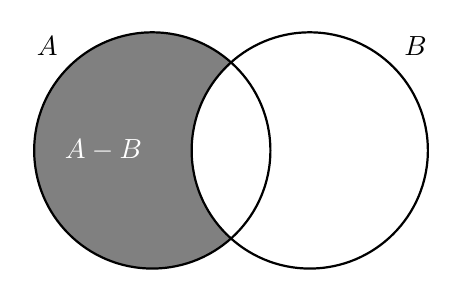
\begin{tikzpicture}[thick,
		set/.style = { circle, minimum size = 3cm}]

		% Set A
		\node[set,fill=gray,label={135:$A$}] (A) at (0,0) {};

		% Set B
		\node[set,fill=white,label={45:$B$}] (B) at (0:2) {};

		% Circles outline
		\draw (0,0) circle(1.5cm);
		\draw (2,0) circle(1.5cm);

		% Difference text label
		\node[left,white] at (A.center){$A-B$};
\end{tikzpicture}
\end{center}

\end{answer}
        
\begin{problem}[{3}]
	Simplify the following expressions to their minimal expressions:
	\begin{enumerate}
		\item $\bar{x}\cdot(\bar{y} + \bar{z}) \cdot (x + y + \bar{z})$
		\item $\bar{a} \cdot b \cdot (\bar{d} + \bar{c} \cdot d) + b \cdot (a + \bar{a} \cdot c \cdot d)$
	\end{enumerate}
    Given: FILL THIS IN \\
    Find: FILL THIS IN
\end{problem}
\begin{answer}
    TODO
\end{answer}
        
\begin{problem}[{4}]
Derive the simplest sum-of-products expression for the function $f(x_1, x_2, x_3, x_4) = x_1\bar{x}_3\bar{x}_4 + x_2\bar{x}_3x_4 + x_1\bar{x}_2\bar{x}_3$. \\
    Given: FILL THIS IN \\
    Find: FILL THIS IN
\end{problem}
\begin{answer}
    TODO
\end{answer}
        
\end{document}
